% =============================================================================
% READY-TO-PASTE LaTeX SECTIONS FOR GROUP 3 REPORT (report.pdf)
% Author: Hua Tue Minh (Computer Science - Group 3, Mentor Pod 1, HCMUT)
% Covers:
%   - Section 2.4: Control Logic: Two-Level Constrained MPC
%   - Section 4.1: PLC Hard Safety Guardrails and Fail-Safe Fallback Matrix
%   - Section 4.2: Operator Monitoring Dashboard
%
% Every number below is read from poc_simulation/results/ (committed run) or from
% poc_simulation/analysis_l4_decomposition.py (results/real_l4_staging_decomposition.csv).
%
% Required packages: amsmath, booktabs, graphicx (already loaded) + array (add \usepackage{array}
%   to the preamble; it provides >{\raggedright\arraybackslash} for the fallback table).
% Required figures (copy from poc_simulation/figures/ into Overleaf figures/):
%   5. fig5_dashboard_fault_test.png
%   6. fig6_dashboard_comparison.png
%
% Citation keys to add to the bibliography if not present:
%   skogestad2003  S. Skogestad, "Simple analytic rules for model reduction and PID
%                  controller tuning," J. Process Control, 13(4), 291-309, 2003.
%   isa101         ANSI/ISA-101.01-2015, Human Machine Interfaces for Process
%                  Automation Systems.
% =============================================================================

% -----------------------------------------------------------------------------
% PASTE UNDER CHAPTER 2 -> after Section 2.3
% -----------------------------------------------------------------------------
\section{Control Logic: Two-Level Constrained Model Predictive Control}
\label{sec:mpc}

The forecasts of Section~\ref{sec:forecasting} are consumed by two controllers that act on different time scales. A \textbf{Zone-Level MPC} recomputes the dry-cooling-coil (DCC) duty $u = \dot{Q}_{\text{DCC,cmd}}$ every minute over a 15-minute horizon, and a \textbf{Plant-Level Chilled-Water (CHW) Coordinator} resets the DCC supply temperature $T_{\text{CHW}}$ every 15 minutes. Three supervisory rules (L1--L3) run alongside both. All of this logic is implemented in \texttt{poc\_simulation/controllers.py} and is identical for \texttt{SensorOnly\_MPC} and \texttt{EquipState\_MPC}; the two variants differ only in which forecast they receive and in their estimate of the current load (an S23 sub-meter reading with $0.8\text{ kW}$ noise for Equipment-State, a BMS estimate with a 2-minute lag and $2.5\text{ kW}$ noise for Sensor-Only).

\subsection{Prediction Model and Quantile Disturbance Trajectories}

Inside the optimiser, the zone energy balance of Eq.~(3.12) is discretised at $\Delta t = 60\text{ s}$, with the actuation lag of Eq.~(3.14) represented by a $d = \tau_{\text{dead}} = 4$-step transport queue followed by a first-order coil lag:
\begin{align}
T_z^{(q)}(k+1) &= T_z^{(q)}(k) + \frac{\Delta t}{C_{\text{eff}}}\Big[\dot{Q}_{\text{env}} + \dot{Q}^{(q)}_{\text{room}}(k) + \dot{Q}_{\text{aux}} + \dot{Q}_{\text{MAU,adv}} - \dot{Q}_{\text{DCC}}(k)\Big], \label{eq:mpc_T}\\
\dot{Q}_{\text{DCC}}(k+1) &= \dot{Q}_{\text{DCC}}(k) + \alpha\big(u(k-d) - \dot{Q}_{\text{DCC}}(k)\big), \qquad \alpha = 1 - e^{-1/\tau_{\text{coil}}}, \label{eq:mpc_coil}
\end{align}
where $q \in \{10, 50, 90\}$ indexes the forecast quantile. The envelope and MAU advection terms are held at their current values across the horizon. Each disturbance trajectory $\dot{Q}^{(q)}_{\text{room}}(k)$, $k = 1,\dots,15$, is linearly interpolated through the current load estimate and the calibrated $h = 5, 10, 15\text{ min}$ quantiles, mapped from HIPE kW to bay kW by the affine bay mapping of Section~3.2. The same command sequence is therefore rolled out three times: once under the median load and once under each tail.

\subsection{Zone-Level Optimisation Problem}

To keep the problem small enough for a PLC-adjacent edge computer, the 15 future moves are blocked into three decision variables ($u(k) = u_0$ for $k = 0..2$, $u_1$ for $k = 3..7$, $u_2$ for $k = 8..14$). The controller minimises
\begin{equation}
\begin{aligned}
J ={}& 4\sum_{k}\big(T_z^{(50)}(k) - 22.05\big)^2
 + 8{\times}10^{-4}\big[(u_0 - u_{\text{prev}})^2 + (u_1 - u_0)^2 + (u_2 - u_1)^2\big]
 + 1.5{\times}10^{-4}\sum_{k} u(k) \\
&+ 450\sum_{k}\big[T_z^{(90)}(k) - 22.88\big]_+^2
 + 450\sum_{k}\big[21.12 - T_z^{(10)}(k)\big]_+^2 \\
&+ 150\sum_{k}\Big(\big[T_z^{(50)}(k) - 22.75\big]_+^2 + \big[21.25 - T_z^{(50)}(k)\big]_+^2\Big)
\end{aligned}
\label{eq:mpc_cost}
\end{equation}
subject to the valve slew limit $|u_0 - u_{\text{prev}}| \le 35\text{ kW/min}$ and the coil capacity bound $0 \le u_i \le UA_{\text{DCC}}\max(0.5,\, T_z - T_{\text{CHW}})$. The four bracketed terms are the \emph{asymmetric quantile chance constraints}: the $P_{90}$ trajectory must stay $0.12\text{ K}$ inside the $23.0^\circ\text{C}$ Tier-2 ceiling, the $P_{10}$ trajectory $0.12\text{ K}$ inside the $21.0^\circ\text{C}$ floor, and the median $0.25\text{ K}$ inside both. The problem is solved with bounded L-BFGS-B (at most 35 iterations), warm-started from the steady-state $P_{50}$ balance, and only $u_0$ is applied before the horizon recedes by one minute.

Two properties of this formulation should be stated plainly. First, the chance constraints are implemented as \emph{soft} quadratic barrier penalties, not as hard constraints, so the solver alone does not guarantee that the Tier-2 band is respected; hard protection is assigned to the PLC layer of Section~\ref{sec:plc}. Second, rolling out the $P_{90}$ load trajectory does not make the resulting temperature a formal 90th percentile; the protection actually delivered is measured empirically, through the $94.0$--$95.1\%$ active upper coverage of Section~\ref{sec:forecasting} and the closed-loop excursion counts of Section~3.2.

\subsection{Plant-Level Chilled-Water Coordinator}

The coordinator sizes $T_{\text{CHW}}$ for the worst load expected over the 15--30-minute chiller staging window:
\begin{align}
\dot{Q}_{\text{peak}} &= \max\!\Big(\max_{k \le 15}\dot{Q}^{(90)}_{\text{room}}(k),\ \dot{Q}^{(90)}_{\text{room}}(30)\Big) + \dot{Q}_{\text{aux}} + \dot{Q}_{\text{env}} + \dot{Q}_{\text{MAU,adv}}, \nonumber\\
T_{\text{CHW}}^{\text{ideal}} &= \operatorname{clip}\!\Big(T_{\text{target}} - \frac{\dot{Q}_{\text{peak}}}{UA_{\text{DCC}}} - 0.45,\ 11.8,\ 16.5\Big),
\label{eq:chw}
\end{align}
where the $0.45\text{ K}$ term preserves valve authority. The set-point is updated every 15 minutes, or immediately if $T_{\text{CHW}}^{\text{ideal}}$ falls more than $0.4\text{ K}$ below the current command (pre-chill override), and each update is limited to $+1.2\text{ K}$ or $-2.0\text{ K}$. On the peak test day the Equipment-State coordinator held a mean $T_{\text{CHW}} = 14.64^\circ\text{C}$ (range $12.11$--$15.24^\circ\text{C}$) against the static $12.0^\circ\text{C}$, which raises DCC chiller COP by about $3\%$ per kelvin (Section~3.3.1).

The coordinator also applies a \textbf{standby-staging credit} $\varepsilon$ to chiller power, $P_{\text{chiller}} \leftarrow (1 + \varepsilon)\,P_{\text{chiller}}$, intended to represent the spinning reserve a static plant must hold against unforecast swings:
\begin{equation}
\varepsilon = -\min\!\big(0.065,\ 0.24\,\max(0,\ 1.35f - \bar{s}/\dot{Q}_{\text{ref}})\big),
\label{eq:credit}
\end{equation}
where $\bar{s}$ is the mean $P_{90} - P_{50}$ spread at 15 and 30 minutes and $\dot{Q}_{\text{ref}} = 219.24\text{ kW}$. This term is a parametric assumption, not a simulated staging sequence, and it scales with the fluctuation regime $f$ by construction. Table~\ref{tab:l4_decomp} separates it from the physically simulated CHW-reset gain.

\begin{table}[htbp]
\centering
\caption{Decomposition of the Isolated Pure-L4 Chiller Saving $s_4$ (Equip-State MPC, L1--L3 Locked, Real HIPE Dec~6, 2017)}
\label{tab:l4_decomp}
\small
\begin{tabular}{@{}lcccc@{}}
\toprule
\textbf{Regime $f$} & \textbf{Total $s_4$} & \textbf{CHW-Reset COP Gain} & \textbf{Staging Credit (Eq.~\ref{eq:credit})} & \textbf{Workbook Prior} \\
\midrule
5\%  & 3.36\% & 2.26\% & 1.10\% & 2.50\% \\
10\% & 5.60\% & 3.41\% & 2.20\% & 5.00\% \\
20\% & 9.06\% & 4.47\% & 4.59\% & 10.00\% \\
\bottomrule
\end{tabular}
\end{table}

The physically simulated part of L4 reaches $2.26$--$4.47\%$ of chiller electricity, and the agreement of total $s_4$ with the workbook prior $0.5f$ depends on the staging credit, which supplies $39\%$ of $s_4$ at $f = 10\%$ and about half at $f = 20\%$. In the full Scenario~A2 ablation the credit accounts for $1.80\text{ kW}$ of the $32.92\text{ kW}$ average reduction, about $1.1$ percentage points of the $20.28\%$ headline saving. Replacing Eq.~(\ref{eq:credit}) with a chiller staging model fitted to plant data is the first item of future work.

\subsection{Supervisory Rules L1--L3}

The three rules use MES/GEM context directly and are identical in both MPC variants, so the ablation isolates the value of the forecast:
\begin{itemize}
    \item \textbf{L1, MSL-aware dew-point reset:} the MAU coil exit is held at $8.6^\circ\text{C}$ whenever an $\text{MSL} \ge 3$ lot is open or scheduled to open within the next 75 minutes (more than $2\tau_w \approx 63\text{ min}$ ahead, so the zone has dried before the lot opens), and relaxed to $10.5^\circ\text{C}$ otherwise.
    \item \textbf{L2, load-aware reheat bypass:} electric reheat is bypassed when at least 60\% of tools are in RUN and the zone is above $21.35^\circ\text{C}$.
    \item \textbf{L3, FFU turndown:} recirculation drops from 35 to 30~ACH when fewer than 60\% of tools are in RUN and the MES schedule shows fewer than 65\% in RUN 10 minutes ahead, so full airflow is restored before production resumes.
\end{itemize}
On the peak test day both MPC variants spent the same 592 minutes with the MAU coil below $8.8^\circ\text{C}$, 403 minutes with electric reheat off and 989 minutes at 30~ACH, confirming that the L1--L3 actuation was identical across the ablation.


% -----------------------------------------------------------------------------
% PASTE UNDER CHAPTER 4 -> \section{...PLC Hard Safety Guardrails...}
% -----------------------------------------------------------------------------
\section{PLC Hard Safety Guardrails and Fail-Safe Fallback Matrix}
\label{sec:plc}

The MPC of Section~\ref{sec:mpc} is an optimiser that runs on top of the facility PLC; it does not replace it. A guardrail layer evaluated before every control step owns the hard limits and works without any forecast, so that a wrong forecast, a lost MES link or a failed actuator degrades the system to today's static practice rather than to an unsafe state. Table~\ref{tab:fallback} summarises the three mechanisms and their validation on the peak test day.

\begin{table}[htbp]
\centering
\caption{Fail-Safe Fallback Matrix and Validation Under Three Injected 60-Minute Faults (Real HIPE Dec~6, 2017, Scenario A2)}
\label{tab:fallback}
\small
\renewcommand{\arraystretch}{1.12}
\begin{tabular}{@{}>{\raggedright\arraybackslash}p{2.7cm}>{\raggedright\arraybackslash}p{3.6cm}>{\raggedright\arraybackslash}p{4.3cm}>{\raggedright\arraybackslash}p{3.9cm}@{}}
\toprule
\textbf{Fault} & \textbf{Detection} & \textbf{PLC Response} & \textbf{Validation Result} \\
\midrule
Zone sensor drift (Sensor~1 $+1.8\text{ K}$, $+6\%$ RH, 09:30--10:30) &
Any of three sensors deviates from the median by $>0.6\text{ K}$ or $>2.5\%$ RH &
Outlier excluded; control uses the mean of the agreeing sensors &
Isolated 60/60~min; measured-temperature error $\le 0.12\text{ K}$ \\
\addlinespace
SECS/GEM link loss (13:00--14:00), or Tier-1 margin reached &
Missing heartbeat, or $T \le 20.3$ / $\ge 23.7^\circ\text{C}$, RH $\le 36.5$ / $\ge 53.5\%$ &
Bumpless transfer to SIMC PID~\cite{skogestad2003} ($K_p = 55$, $K_i = 0.45$, $K_d = 180$) with static safe set-points ($8.6^\circ\text{C}$ coil, $21.0^\circ\text{C}$ reheat, 35~ACH, $12.0^\circ\text{C}$ CHW) &
Fallback 60/60~min; first PID command within $25.7\text{ kW}$ of the last MPC command; $T_z \in [21.68, 22.32]^\circ\text{C}$ \\
\addlinespace
Cooling valve stuck at 78\% authority (15:30--16:30) &
Commanded duty exceeds delivered duty by $>5\text{ kW}$ &
CHW forced to $11.8^\circ\text{C}$ and FFU restored to 35~ACH &
Active 60/60~min; $T_z \le 22.34^\circ\text{C}$ \\
\bottomrule
\end{tabular}
\end{table}

\textbf{Bumpless transfer.} When the fallback engages, the PID integrator is initialised to the last MPC command plus the sensible step caused by re-arming MAU reheat, $\dot{m}_{\text{MAU}}c_p(21.0 - T_{\text{MAU,sa}})$, so the coil duty does not jump when the static reheat set-point returns. The PID output is rate-limited to $30\text{ kW/min}$. When the trigger clears, the MPC resumes from the PID's last command, which makes the return transfer bumpless as well.

\textbf{Combined result.} With all three faults injected on the peak day, the Equipment-State MPC with guardrails recorded \textbf{0~minutes of Tier-1 and 0~minutes of Tier-2 violation} ($T_z \in [21.58, 22.84]^\circ\text{C}$, $\text{RH}_{\max} = 44.09\%$ during $\text{MSL} \ge 3$). The voting logic raised no false alarm in the three fault-free 24-hour runs (0 of 4,320 controller-minutes).

\textbf{Limits of this validation.}
\begin{itemize}
    \item The $<1\text{ s}$ transfer time is a requirement on the PLC scan cycle. The simulator advances in 1-minute steps, so it demonstrates transfer within one control step, not sub-second timing.
    \item In the fault test the fallback was triggered only by the link loss. The Tier-1-margin trigger was never reached in any run, so that path is implemented but not yet exercised.
    \item Median voting catches a single sensor that moves by more than $0.6\text{ K}$. A slow drift below that threshold, or a common-mode error affecting all three sensors, would pass undetected; periodic calibration against a reference instrument is still required.
    \item The valve fault is a parameterised capacity cap motivated by the LBNL fault days, not a replay of LBNL trajectories.
    \item The guardrails protect Tier-1, not Tier-2. Under a $-20\%$ plant--model mismatch the Equipment-State MPC still spent 2~minutes above $23.0^\circ\text{C}$ (peak $23.03^\circ\text{C}$), and in the isolated-L4 sweep at $f = 20\%$ it spent 6~minutes above the band (Section~3.2), in both cases without any Tier-1 breach.
\end{itemize}


% -----------------------------------------------------------------------------
% PASTE UNDER CHAPTER 4 -> \section{...Operator Monitoring Dashboard...}
% -----------------------------------------------------------------------------
\section{Operator Monitoring Dashboard}
\label{sec:dashboard}

Operators will only trust a forecast-driven controller if they can see what it is doing and why. We therefore built a monitoring dashboard (\texttt{dashboard/app.py}, Streamlit with Altair charts) that replays the minute-by-minute simulator output of Section~3.2 as a control-room view. It reads the result files directly, so every figure on screen comes from the simulation; nothing is entered by hand.

\textbf{Design principles.} The layout follows the high-performance HMI approach of ISA-101~\cite{isa101}: the screen stays in neutral greys while the bay is normal, colour appears only for an abnormal state (amber for an expected abnormal condition such as an open $\text{MSL} \ge 3$ lot or a PID fallback, red for a limit breach or detected fault), and every colour is paired with a word, so the display remains readable for colour-blind operators and on a monochrome printout. Only the proposed controller is drawn in the accent colour; reference controllers are drawn in greys. Each temperature and humidity chart shows the trace inside its shaded Tier-2 envelope, which is the one image an operator needs to judge whether the bay is safe.

\textbf{Three views.}
\begin{enumerate}
    \item \textbf{Live operation:} a time slider replays the 24-hour day for any of the three controllers, with four figures (zone temperature, RH, HVAC power, energy saved so far, each with its margin stated in words), a bay-status column and the temperature and RH envelopes.
    \item \textbf{PLC fault test} (Figure~\ref{fig:dash_fault}): the same view on the three-fault run, adding sensor-voting, control-mode and valve status, the raw drifting Sensor~1 reading while it is excluded, and an \textbf{event log} generated from the simulator flags that lists each abnormal state with its start, end, duration and the guardrail response.
    \item \textbf{Controller comparison} (Figure~\ref{fig:dash_compare}): the three controllers overlaid on the 10:12 \texttt{ChipPress} surge against the $23.0^\circ\text{C}$ limit, the 24-hour summary table and the annual electricity split by chillers, reheat and fans.
\end{enumerate}

\begin{figure}[htbp]
    \centering
    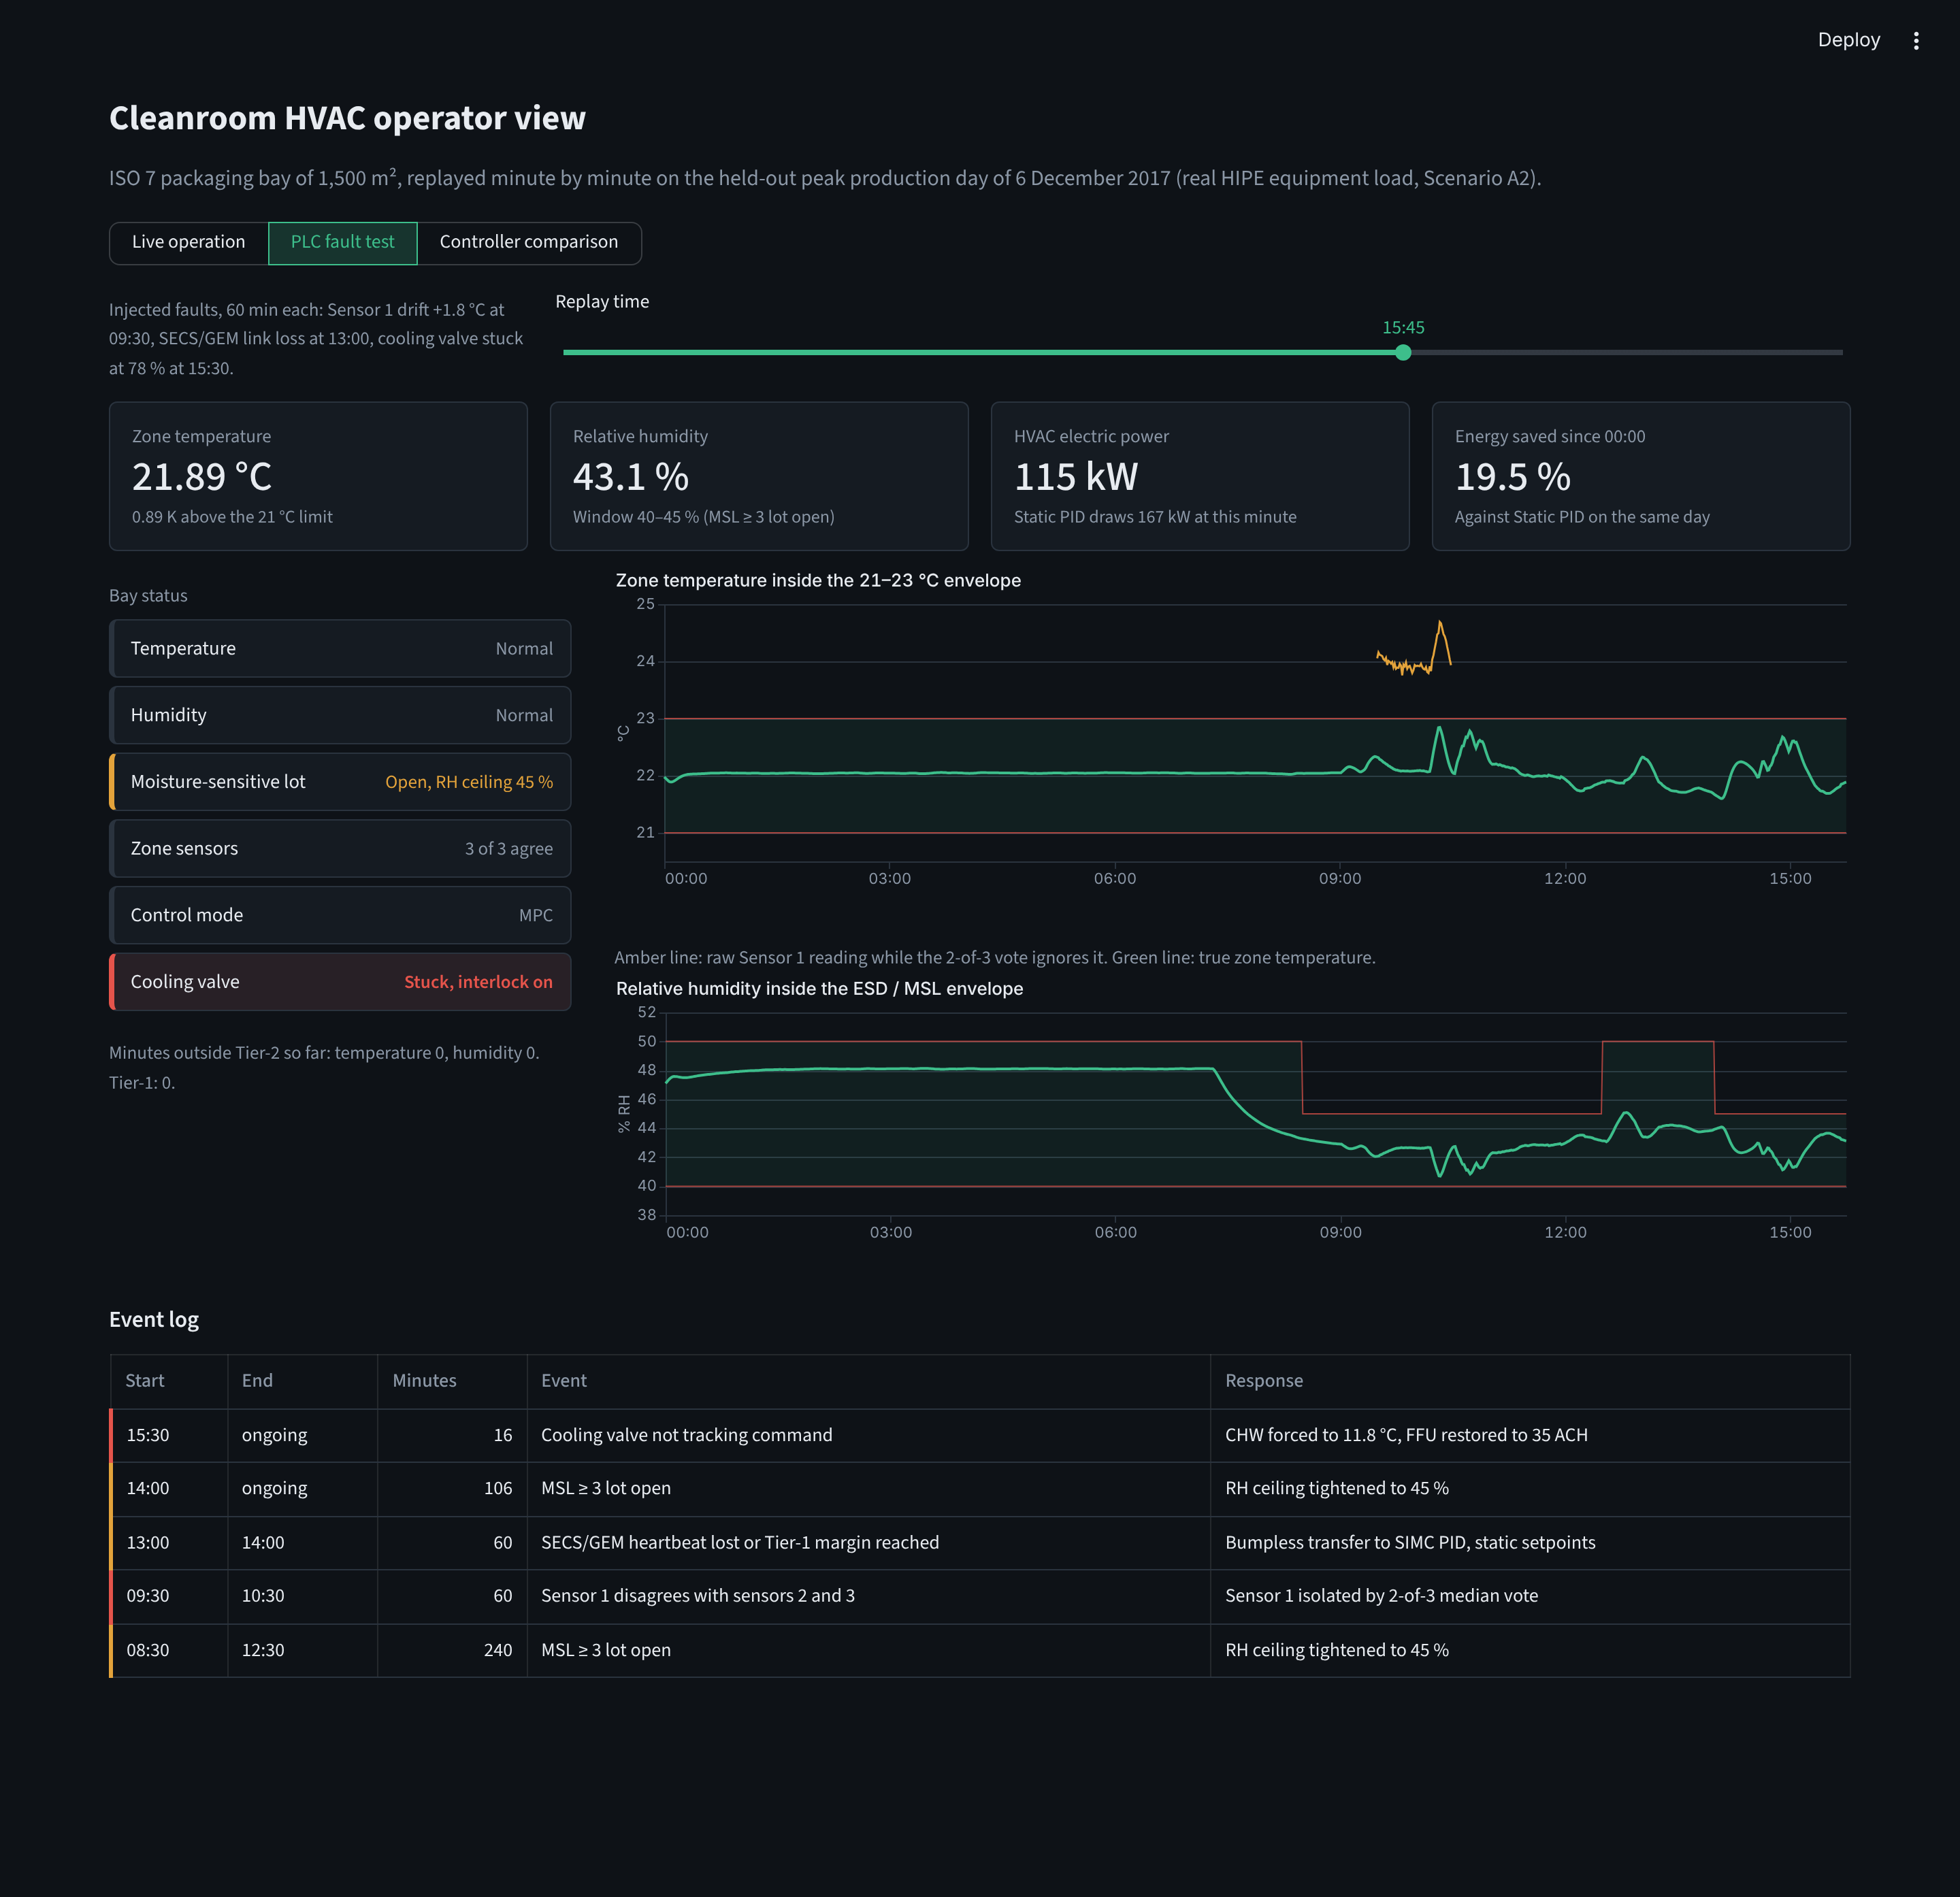
\includegraphics[width=\textwidth]{figures/fig5_dashboard_fault_test.png}
    \caption{Operator dashboard, PLC fault test view at 15:45 on Dec~6, 2017: the cooling-valve interlock is active (red), an $\text{MSL} \ge 3$ lot is open (amber), and the event log lists the earlier Sensor~1 isolation and SECS/GEM fallback with the guardrail response to each.}
    \label{fig:dash_fault}
\end{figure}

\begin{figure}[htbp]
    \centering
    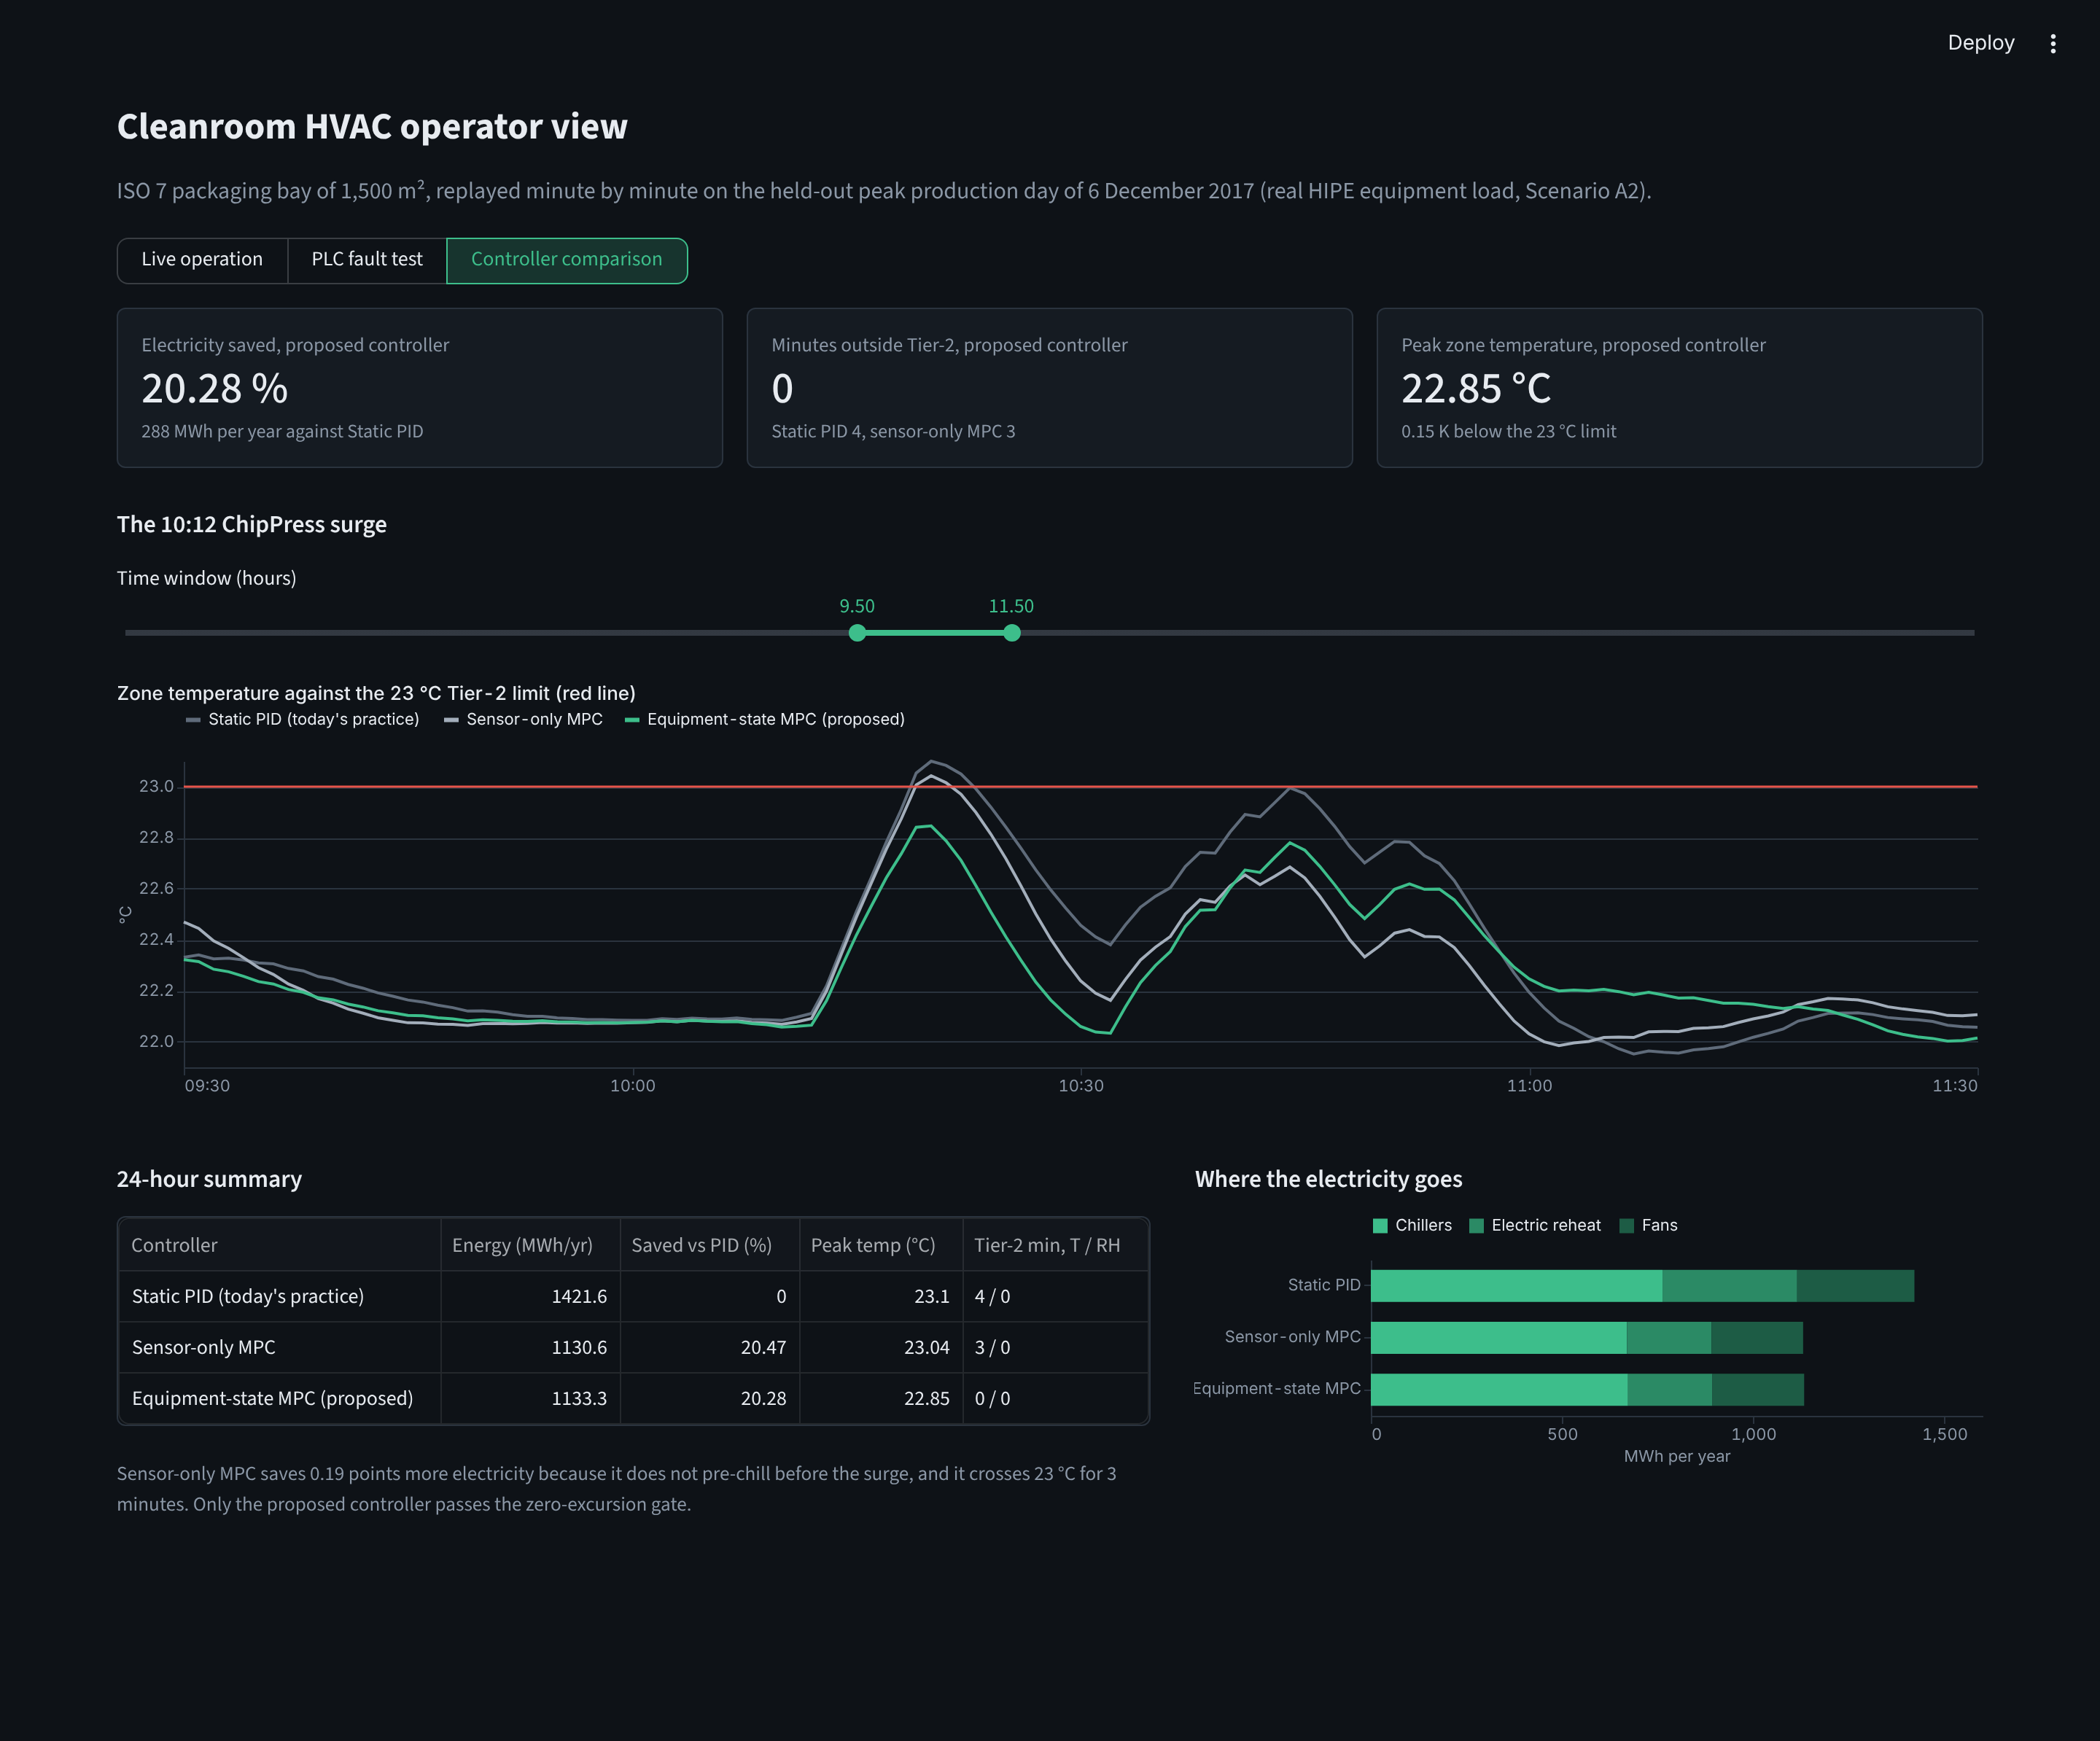
\includegraphics[width=\textwidth]{figures/fig6_dashboard_comparison.png}
    \caption{Operator dashboard, controller comparison view: only the Equipment-State MPC (green) stays below the $23.0^\circ\text{C}$ limit through the 10:12 surge while saving $20.28\%$ of HVAC electricity against Static PID.}
    \label{fig:dash_compare}
\end{figure}

\textbf{From prototype to plant.} The prototype reads CSV files; in a plant the same views would subscribe to the BMS historian and the MES event stream (for example over OPC~UA), and the event log would be written by the PLC itself. The dashboard is a monitoring tool only: it issues no commands, so it adds no new path by which the bay could be driven out of specification.
